\chapter{Background}

\section{GPU Computing}

To understand how GPU software works, it’s important to first understand GPU hardware since the code used to program GPUs aligns very closely with the underlying hardware. Today’s GPUs have many fundamental design decisions that may seem unfamiliar when compared to that of a CPU’s architecture. This paper uses AMD's GCN architecture as an example for many of the GPU metrics and comparisons. This is due to the fact that the GCN architecture is an extremely prevalent GPU architecture, and it is the main architecture currently supported by AMD's ROCm ecosystem. This includes the Radeon Vega Pro cards with the 2017 GCN 5 architecture that was used for this thesis' tests and experiments. As of November 2021, ROCm has expanded its list of supported devices to include the AMD Radeon Pro W6800 GPU which was released in 2020 and uses the newer RDNA 2 architecture \cite{rocmCompatibility}. We hope that in the near future, ROCm will continue to evolve and support new GPU architectures and devices.

\subsection{Modern GPU Architecture}

The fundamental building block of all modern GPU designs are clusters of processing elements grouped together with resources. AMD refers to these processing groups as Compute Units (CUs) which can be equated with the term Streaming Multiprocessors (SMs) on CUDA capable GPUs \cite{amdConferenceTalk}. AMD's GCN architecture groups many of these CUs into processors called Shader Units that are each managed with their own Workload Manager as seen in Figure \ref{gcn2}. Each Compute unit has its own resources such as a scalar unit for flow control, cache memory, registers, and more. The main computation unit for each CU is a collection of vector units, or Streaming Processors in CUDA terminology, that share an instruction cache. These vector units can be conceptually thought of as SIMD (Single Instruction/Multiple Data) units that are capable of performing floating point calculations since each SIMD contains its own a floating point unit. They are capable of treating arrays of data as single elements through which an operation should be applied across. In AMD’s GCN architecture, each Compute Unit is divided up into four SIMD units where each unit is 16 lanes wide and therefore capable of simultaneously executing a single operation across 16 work items \cite{gcnWhitepaper}. This gives us a throughput of 64 single-precision operations per-cycle on each CU.

\begin{figure}[hbtp]
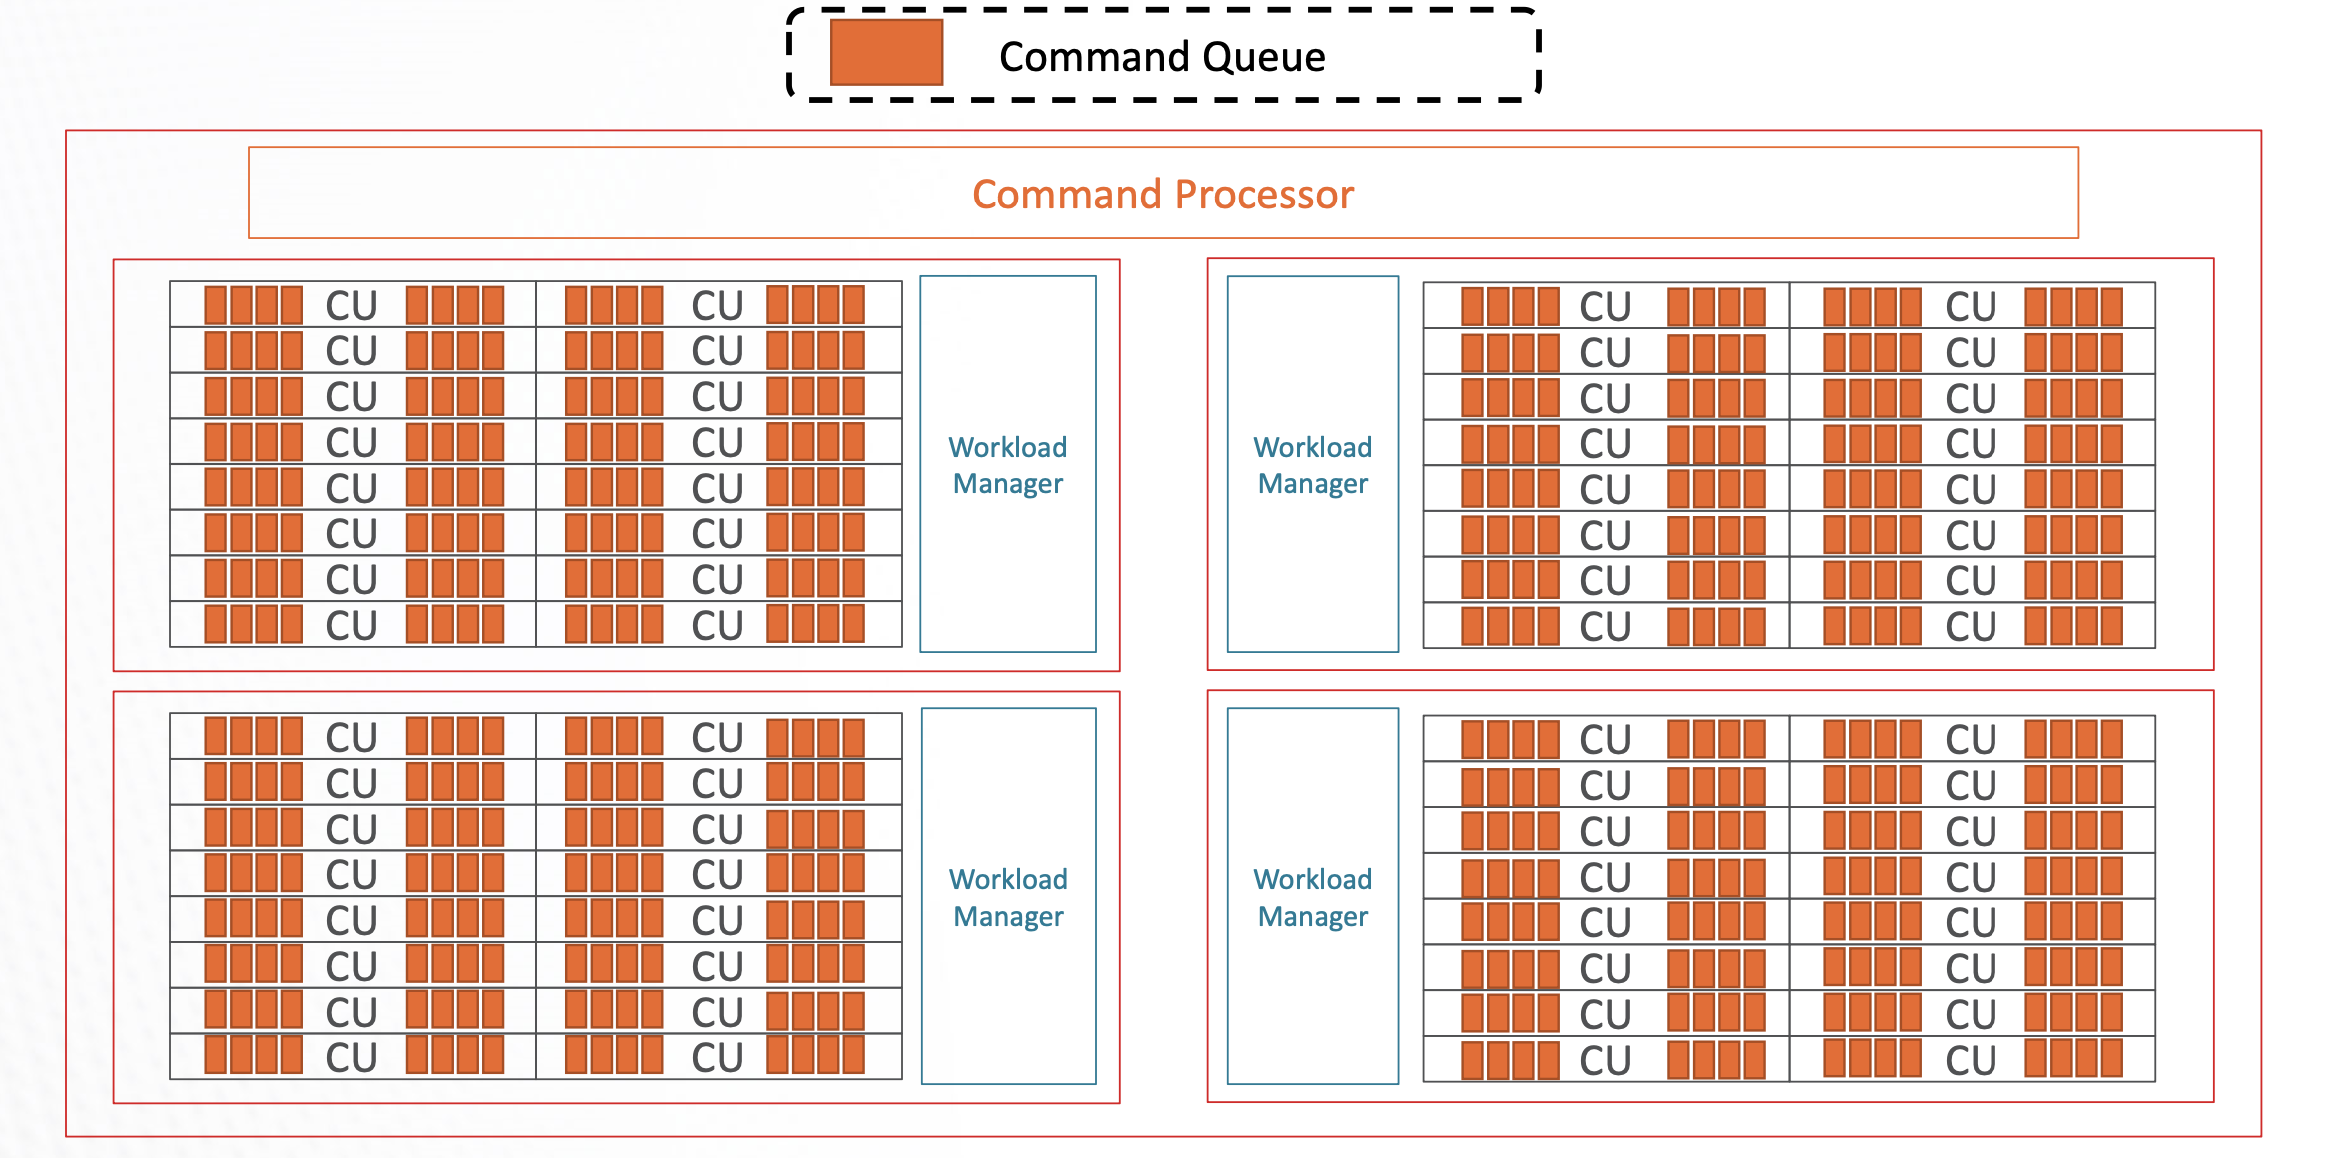
\includegraphics[width=\textwidth]{figures/gcn2.png}
\centering
\caption{A GCN-based AMD GPU that groups Compute Units into Shader Engines that are each managed by a Workload Manager \cite{amdConferenceTalk}.}
\label{gcn2}
\end{figure}

\quad Threads within a GPU are not scheduled individually. Instead, threads are grouped into units called wavefronts on AMD devices or warps for CUDA devices. Wavefront size is a property of the hardware architecture. They are 64 threads wide for GCN-based architectures, for example, or 32 threads wide on NVIDIA's CUDA-capable architectures. Wavefronts are executed on a single SIMD in four consecutive cycles. A one-cycle instruction therefore is executed in four batches across the each of the four 16-lane-wide SIMD units to cover all 64 lanes in an AMD wavefront. This hierarchy of CUs, SIMD units, wavefronts, and threads is illustrated in Figure \ref{gcn1}. 

\begin{figure}[hbtp]
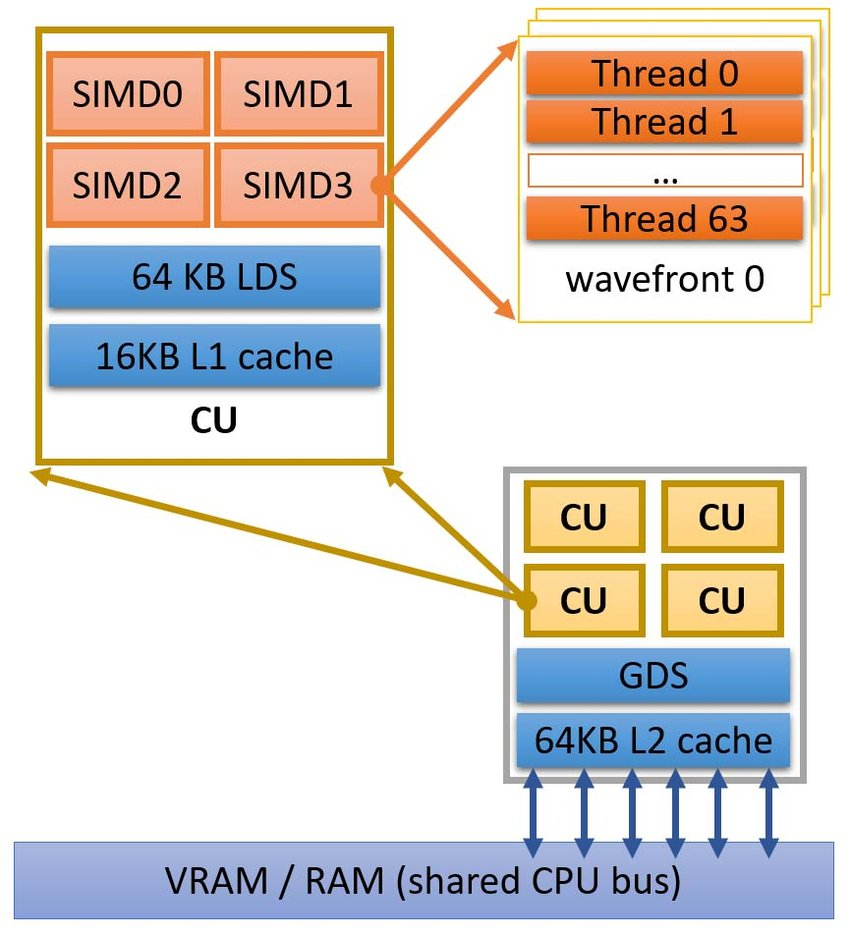
\includegraphics[width=70mm,scale=0.5]{figures/gcn1.png}
\centering
\caption{The contents of a Compute Unit is divided up into a group of resources and SIMD units that are each in turn separated out into wavefronts and threads \cite{gpuSortPerformance}.}
\label{gcn1}
\end{figure}


\quad GPU architectures are further complicated by their multi-tier hierarchy of memory. Visible to all CUs on the entire GPU is gigabytes of Graphics Double Data Rate (GDDR) synchronous DRAM and sometimes High-Bandwidth Memory (HBM) on newer devices. This memory is collectively referred to as `global memory'. When compared to CPU DRAM, the off-chip global memory for GPUs is designed for high bandwidth due to characteristics of the data commonly used for GPU acceleration. Unfortunately, global memory is still susceptible to longer latency times which is a fundamental property of the memory type \cite{greenBook, pycuda}. This latency can often act as a bottleneck for GPU acceleration. PCIe controllers help with the transfers across the PCIe bus with host memory, and some devices have Infinity Fabric Controllers that can manage communication with other GPUs on the system. The inclusion of DMA engines allows for asynchronous memory transfers between the device and the host, or between multiple devices. This layout of memory controllers and engines is illustrated in Figure \ref{gcn3}. At a finer level, each compute unit also has its own scratch-pad memory called the Local Data Share (LDS) which is typically 64KB for AMD and NVIDIA architectures. This data share is shared across SIMD units, and it can be used for communication between threads. Accessing shared memory is much faster than global memory, so a variety of techniques exist to help capitalize on this data share during execution time.

\begin{figure}[hbtp]
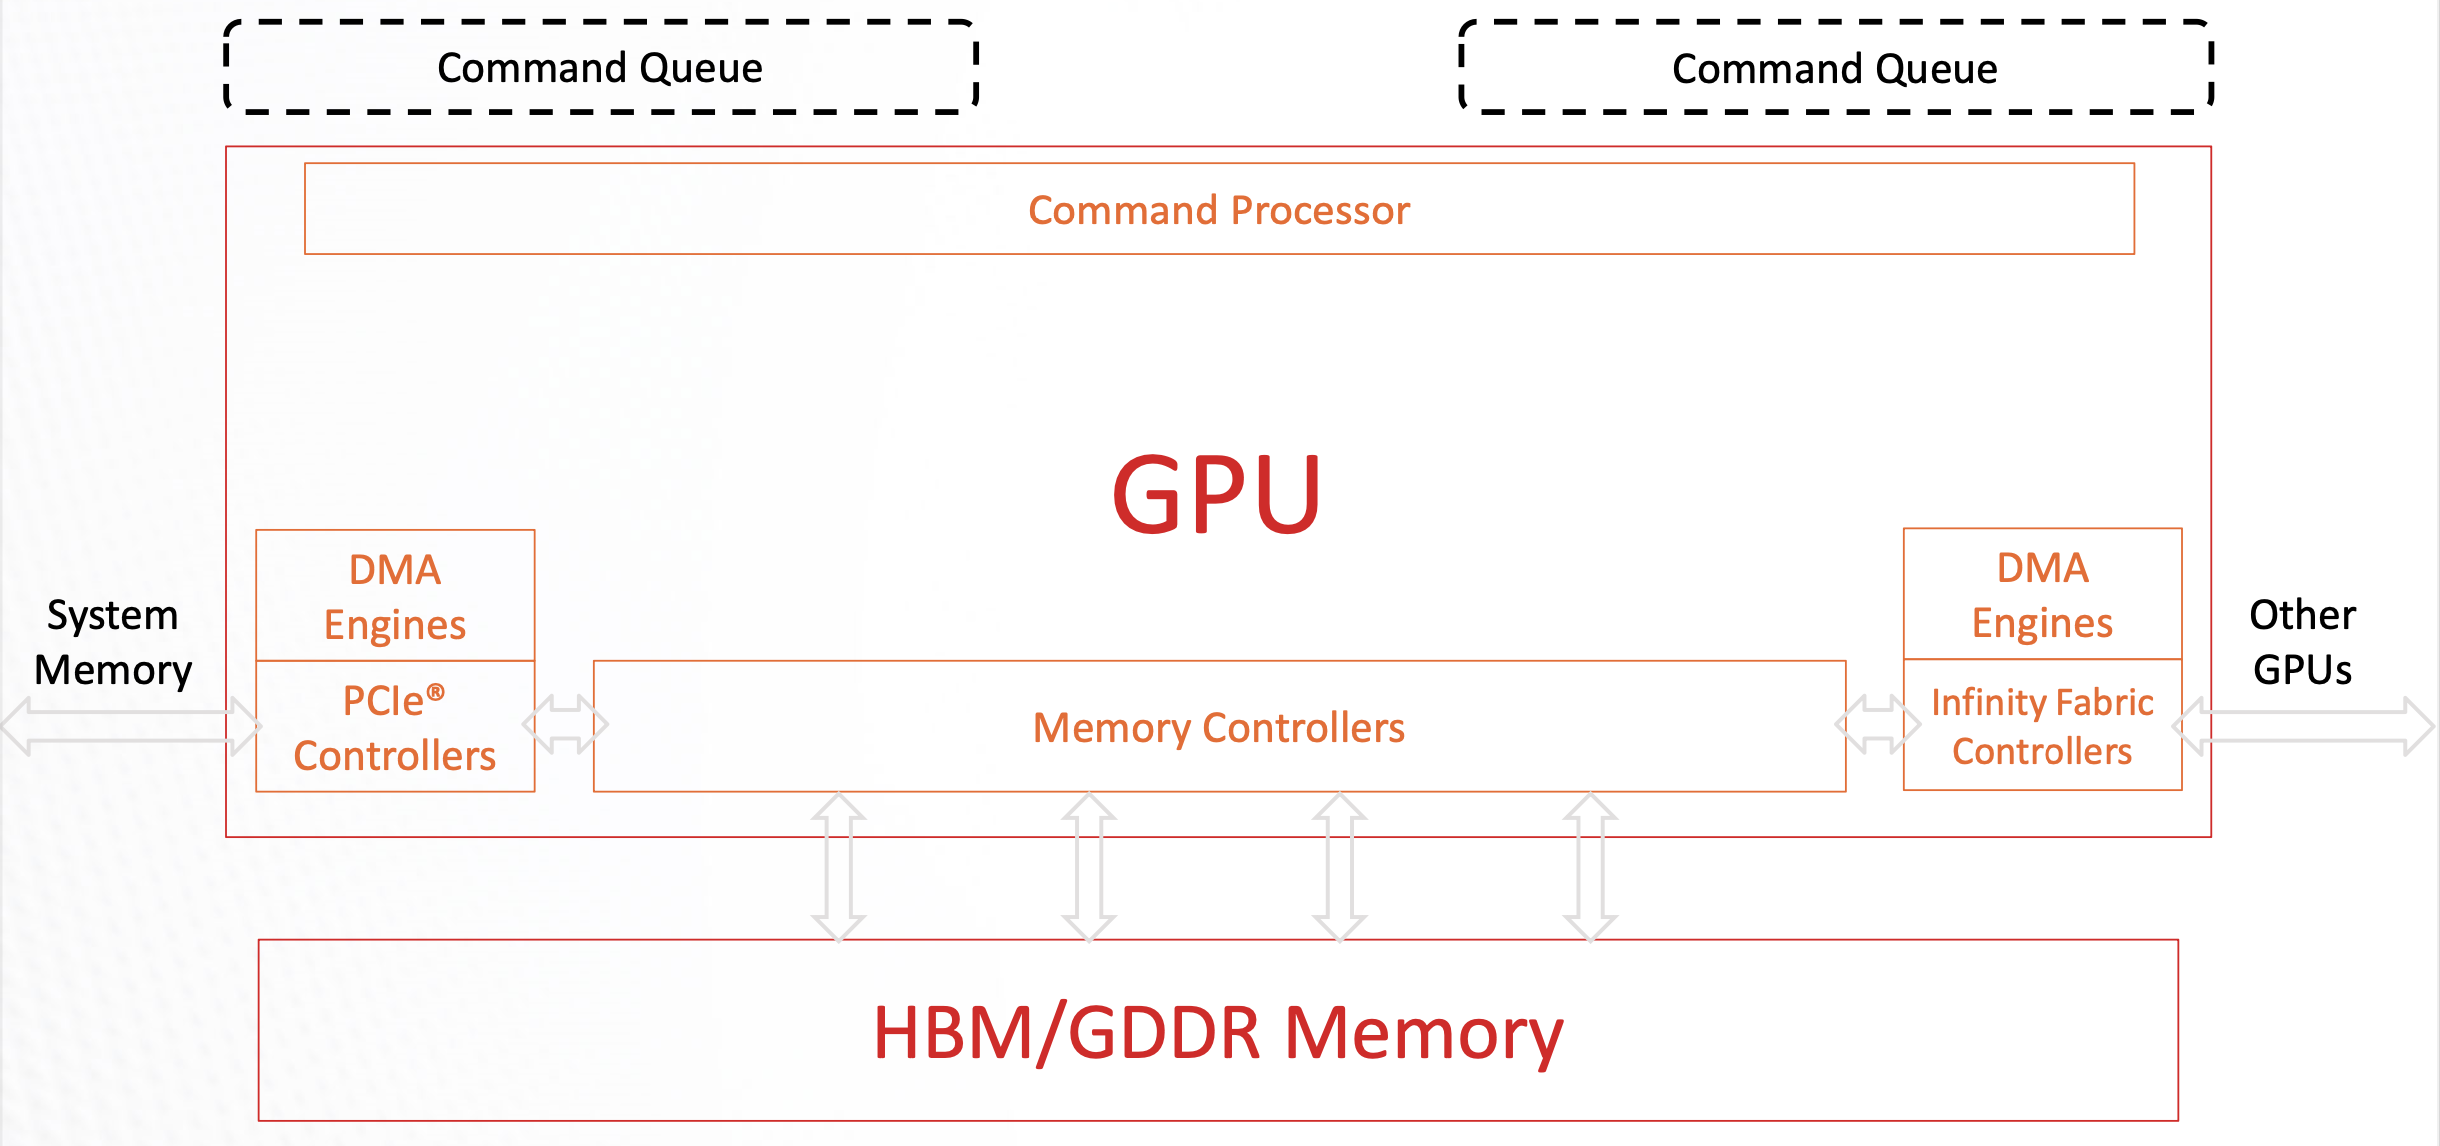
\includegraphics[width=\textwidth]{figures/gcn3.png}
\centering
\caption{A high level overview of the memory architecture on a GCN-based AMD GPU \cite{amdConferenceTalk}.}
\label{gcn3}
\end{figure}

\subsection{GPU Software}

When writing applications that must run on GPUs, code is split into two main parts — host code and device code. Host code is the normal part of an application that will run on the CPU and is written in a standard language such as C++. Device code on the other other hand are functions that are written to be run on SIMD units on a GPU. The entry point to device code sections are functions called kernels. Kernels make use of memory buffers that are allocated on the device from host code in order to manipulate a set of data. This means that most GPU-accelerated applications use a repeating pattern of allocating space on the device, copying data into the memory buffer, running a device kernel, and copying the data back to the host. 

\quad When GPU kernels are launched, they make use of the underlying architecture’s SIMD units to execute the work across many parallel workers which are often referred to as threads. These threads are organized into groups called workgroups on AMD devices or thread blocks on CUDA compatible devices. All threads within a workgroup exist on the device and the CU at the same time. These workgroups are made up of multiple wavefronts as discussed earlier, and GCN hardware uses 16 wavefronts per workgroup. Finally, workgroups are organized into a grid of multiple workgroup blocks as shown in Figure \ref{gridthreadblock}. The number and organization of the blocks and grid are under programmer control within the size limits allowed by the architecture. Blocks can be organized logically into 1, 2, or three dimensional grids, which is usually decided by the topology of the data. Kernels executing on images, for example, often work well as 2-dimensional grids. 

\begin{figure}[hbtp]
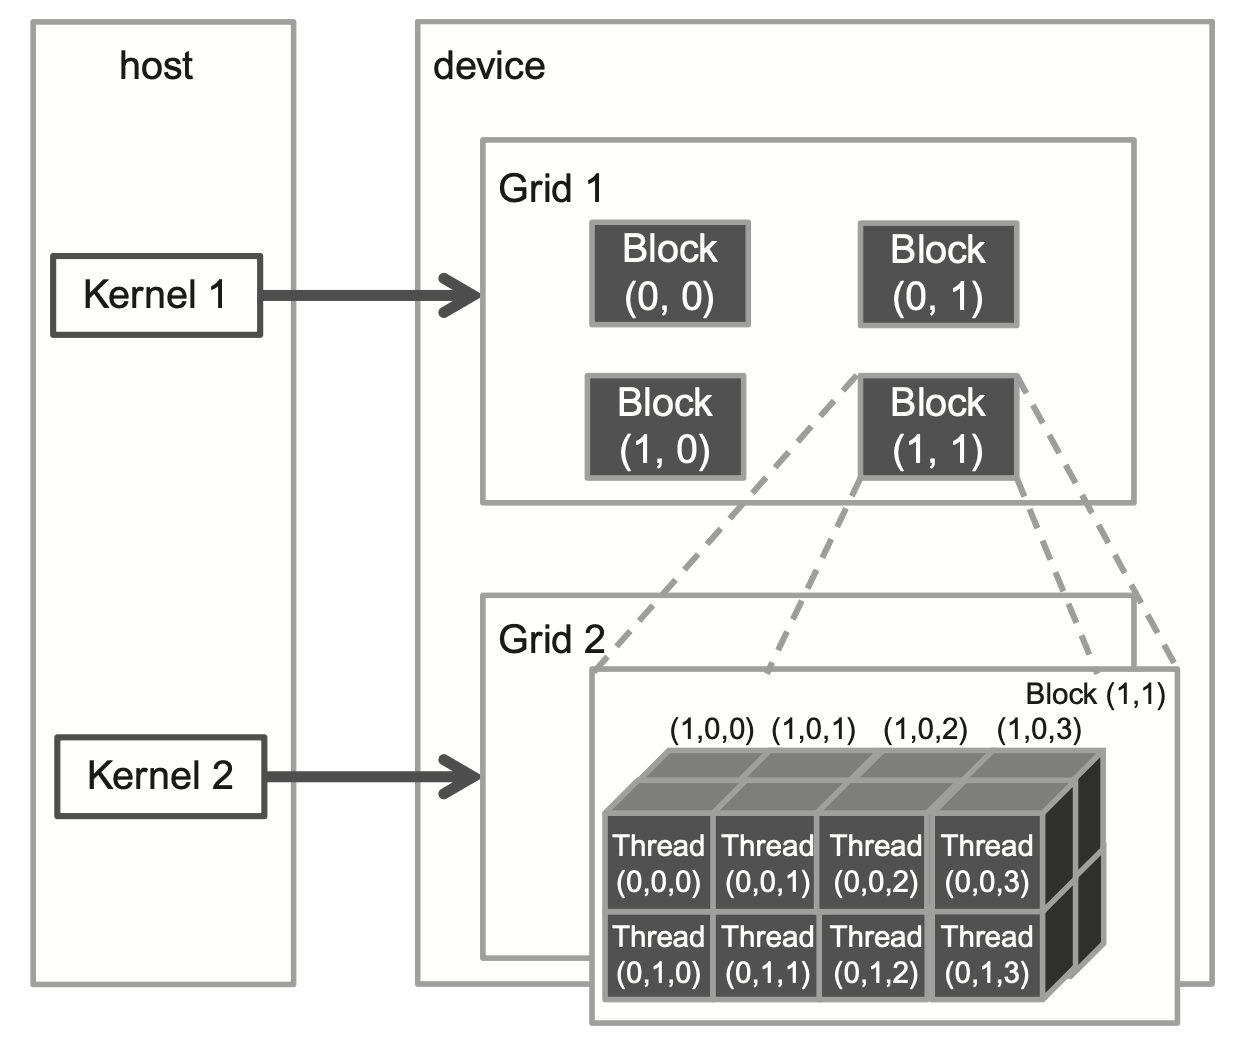
\includegraphics[width=100mm]{figures/gridblockthread.png}
\centering
\caption{GPU kernels divide data elements into logical groupings of grids, threads, and blocks \cite{greenBook}.}
\label{gridthreadblock}
\end{figure}

\quad The hierarchy of grids, blocks, and threads closely matches the organization of the underlying GPU hardware. Blocks are dynamically scheduled onto compute units, and all threads in a block execute on the same compute unit. This allows threads to share LDS memory and L1 cache. The downside to this hierarchy and memory model is that it provides an extra layer of complexity for the programmer. The parameters for the grid and block sizes must be chosen to make use of both the data and the device’s architecture, and kernel code should be designed to take advantage of faster LDS and cache memory when possible to avoid slower access to global memory. 

\quad The final software detail for GPU programming that needs to be discussed are streams. Streams are a way of dividing up the resources of the device for further parallel execution. Streams are queues of tasks that are guaranteed to complete in order on a given stream, and each stream is allowed to overlap and run synchronously with other streams on the same device. The exception to this rule is a special stream known as the null-stream. Tasks in the null-stream are not allowed to overlap with any tasks on any other stream. They only begin execution once all tasks enqueued on all other streams have completed. Blocking calls like memory copies will always happen on the null-stream.


\section{ROCm}

For a long time, NVIDIA has continued to dominate the GPU industry. As of Quarter 2 of 2021, NVIDIA is estimated to hold 83\% marketshare of the discrete GPU market over AMD's 17\% \cite{marketshare}. In the world of GPGPU computing, this dominance has come from its proprietary software included in the CUDA Toolkit which allows for the creation of GPU-accelerated software for embedded systems, workstations, data centers, cloud platforms, and HPC computers \cite{cuda}. This flexibility comes from its compiler, NVCC, which leverages the widely used LLVM infrastructure to allow developers to write kernels in modified syntax in C++ programs and compile them it for execution on NVIDIA devices \cite{nvcc}. On top of this, CUDA's early entry and dominance in the industry has given it the advantage of a strong community and ecosystem. The Radeon Open eCosystem (ROCm) is AMD's answer to CUDA which it describes as its ``open software platform for GPU-accelerated computing'' \cite{rocm}. Launched as part of AMD's ``Boltzmann Initiative'' in 2015, ROCm aims to solve new problems in GPU computing while maintaining an open source and multi-platform identity. This new ecosystem provides a wide range of programming models and languages to choose from. Among those is a C++ dialect called HIP (the Heterogeneous-Computing Interface for Portability) that provides many APIs and interfaces that mirror CUDA's \cite{hip}. It even includes a tool called HIPify that does most, if not all, of the work in converting CUDA programs to HIP. Unlike CUDA which is exclusive to NVIDIA devices, HIP allows for portability across platforms at the expense of a few API limitations \cite{hipfaq}.

\begin{figure}[hbtp]
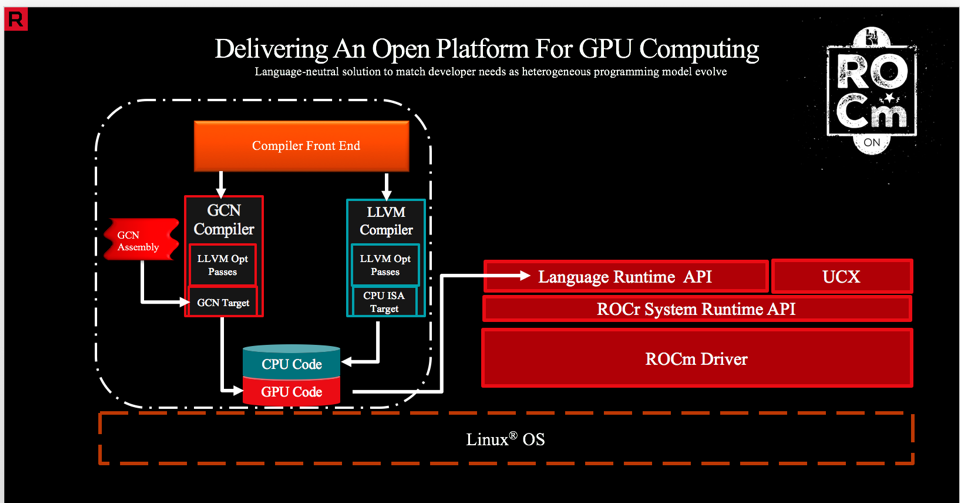
\includegraphics[width=\textwidth]{figures/ROCm_Stack.png}
\centering
\caption{An overview of the various systems in place that make up ROCm's foundation including compilers for both GCN and LLVM-based device runtimes \cite{rocmDocs}.}
\label{rocm1}
\end{figure}

\quad ROCm uses what is called the ROCr runtime which itself is based on the Heterogeneous System Architecture (HSA) Runtime API. The runtime is language-independent which allows it to serve many GPU-compatible languages including AMD's Heterogeneous Compute Compiler (HCC) which provides full control over AMD devices, or the Heterogeneous-Computing Interface for Portability (HIP) which specializes in cross-platform compatibility with both AMD and NVIDIA. To service these languages, the ROCm stack includes both GCN and LLVM compiler toolchains to compile GPU code for all compatible devices. This setup is illustrated in Figure \ref{rocm1}. ROCm also provides a variety of tools for supporting multiple GPUs. The ROCK kernel itself ROCm includes what is known as ROCmRDMA. It allows third party kernel drivers to use direct GPU memory access (DMA) and for DMA-based peer-to-peer data exchanges between devices using PCI express. ROCm also uses the Unified Communication X (UCX) library for both inter-node communication and intra-node communication, as well as the the open source message passing interface OpenMPI. 

\section{Python}

\subsection{Python language}

Python is a dynamically-typed high-level scripting language that has become increasingly popular in recent years. According to Stack Overflow's 2021 Developer Survey, Python gained in popularity over the previous year to become the 3rd most popular language of 2021 with more than 48\% of developers saying they use Python, and the sixth most loved language with more than 67\% of developers expressing interest in continuing to develop with it \cite{soSurvey}. Python has become immensely popular in areas of computing such as machine learning, data analytics, and scientific computing. One of the biggest advantages Python provides is its high level of abstraction and low-verbosity that makes it one of the most concise programming languages -- even when compared with functional languages \cite{rosetta}. This can allow for developers to focus more on high-level designs and processes and less on syntax \cite{pycuda}. When it comes to scientific computing, for example, it has been shown that Python's high level interfaces can help reduce the amount of time that scientists and researchers have to spend writing code \cite{gpucomppy}. 

\quad Python also comes with the advantage of a large compute-ecosystem and many open source libraries available for developers to use. Many libraries for scientific computing have historically been focused on raw performance and achieve this through lower level languages such as Fortran, C, and C++ \cite{pythonEcosystem}. Performance and ease-of-use do not have to be mutually exclusive, however. More recently, library designers have been writing performance-driven code in existing lower-level languages while designing interfaces for this code in a thin layer of Python function-wrappers. The language Python is now becoming synonymous with its massive collection of community-driven libraries and frameworks that tackle just about every computing need imaginable. The most popular of which are open source, open for contributors, and free for programmers to use.



\subsection{CPython}

CPython is the original reference implementation of the Python language. As the name suggests, CPython is implemented in the language C. This is the reason it is so easy for developers to extend the Python language through extension modules written in C or C-compatible languages. Although Python is often described simply as an interpreted language, the CPython implementation includes both a compiler and an interpreter. The compiler generates an AST from the Python source code and compiles it down into bytecode instructions. This bytecode gets executed by CPython's stack-based virtual machine as a giant evaluation loop that terminates once the Python program should stop for any reason.

\quad A very important part of the CPython runtime to understand is the way it handles concurrency. When it comes to maintaining thread-state, the CPython interpreter was created with what is known as the "Global Interpreter Lock" or GIL. It imposes the restriction that only one thread within a given Python process is allowed to process Python bytecode at a time. This means that multi-threading is often restricted to tasks such as IO operations that don't require access to CPython objects, functions, or memory, which all require the GIL to be held \cite{cpythonthreads}. Python programmers often have to turn to multiprocessing to achieve parallelism. Since each process runs in its own instance of the Python interpreter and occupies its own region of memory, each Python process has a distinct GIL instance.

\quad One of the next distinct features of CPython is how it handles Python types. Its easy to generalize Python by saying the language has no types. But in reality, within the CPython implementation, everything has one type -- the ``Python Object'' type. All values, error types, functions, and more are represented as objects that can be stored and passed around. To make this more confusing, every Python object has to be carefully reference-counted for the Python garbage collector to work. When an object is shared or duplicated, this count is incremented. Each time a reference is no longer needed, this count is manually decremented within CPython code. Once the count reaches zero, the Python interpreter knows that the object is no longer needed and its resources can safely be de-allocated. 